\chapter{実験方法}

\section{胃がんの画像データ取得方法}

\subsection{透明化と染色}
はじめに,ホルマリン固定されている検体をLUCIDによる透明化してから染色した.次に検体を蛍光顕微鏡で3D画像として撮影した.LUCIDによる透明化によって,今までは断面のみの撮影だったものを深さ方向まで撮影することを可能にした.本研究で使用した蛍光顕微鏡では,一つの視野で観察することができる領域は縦横が解像度2.49 $\upmu$m/pixで512 pixであるので1.27 mmが一度で見れる視野である.深さ方向はz方向に対して2.7 $\upmu$mの解像度で最大800 $\upmu$mまで観察可能である.縦横の一視野では1.27 mmが撮影されるが,それを検体の長さの分だけ観察するためにタイリングという移動しながら撮影を行う方法で画像を取得した.この際,隣同士の間に余分な空白ができないように画像の15\%を重ねながらタイリングを行った.

\tab {蛍光顕微鏡}に示すような蛍光顕微鏡で撮影を行った.また撮影条件を\tab {レーザー波長}にまとめた.

\begin{table}[H]
	\centering
	\caption{Information of fluorescence microscope}
	\label{tab:蛍光顕微鏡}
	\begin{tabular}{cc}\toprule
		Microscope name & Ti2 Microscope \\ 
		Objective name & Plan Apo 10x \\ 
		Objective magnification & 10 \\ 
		Objective numerical aperture & 0.45 \\ 
		Refractive Index & 1.000 \\
		Z step & 2.7 $\upmu$m \\ \bottomrule
	\end{tabular} 
\end{table}

\begin{table}[H]
	\centering
	\caption{Information of laser wavelength}
	\label{tab:レーザー波長}
	\begin{tabular}{cccc}\toprule
		& DAPI & FITC & Texas Red \\ \midrule
		Emission wavelength (nm) & 440.0--420.0 & 500.0--550.0 & 593.0--670.0 \\ 
		Excitation wavelength (nm) & 405.0 & 405.0 & 561.0 \\ 
		Pinhole size ($\upmu$m) & 20.00 & 20.00 & 20.00 \\ 
		Channel modality & \multicolumn{3}{c}{Laser Scan Confocal, PMT } \\ \bottomrule
	\end{tabular}
\end{table}


\fig {3D検体一覧}に共焦点顕微鏡の撮影した検体の3次元構造を示す.検体ごとに発光波長が異なるのは,染色液の侵食度合い異なることが理由である.

% 三次元に撮影した画像
\begin{figure}[H]
	\centering
	
	\begin{minipage}{0.45\columnwidth}
		\centering
		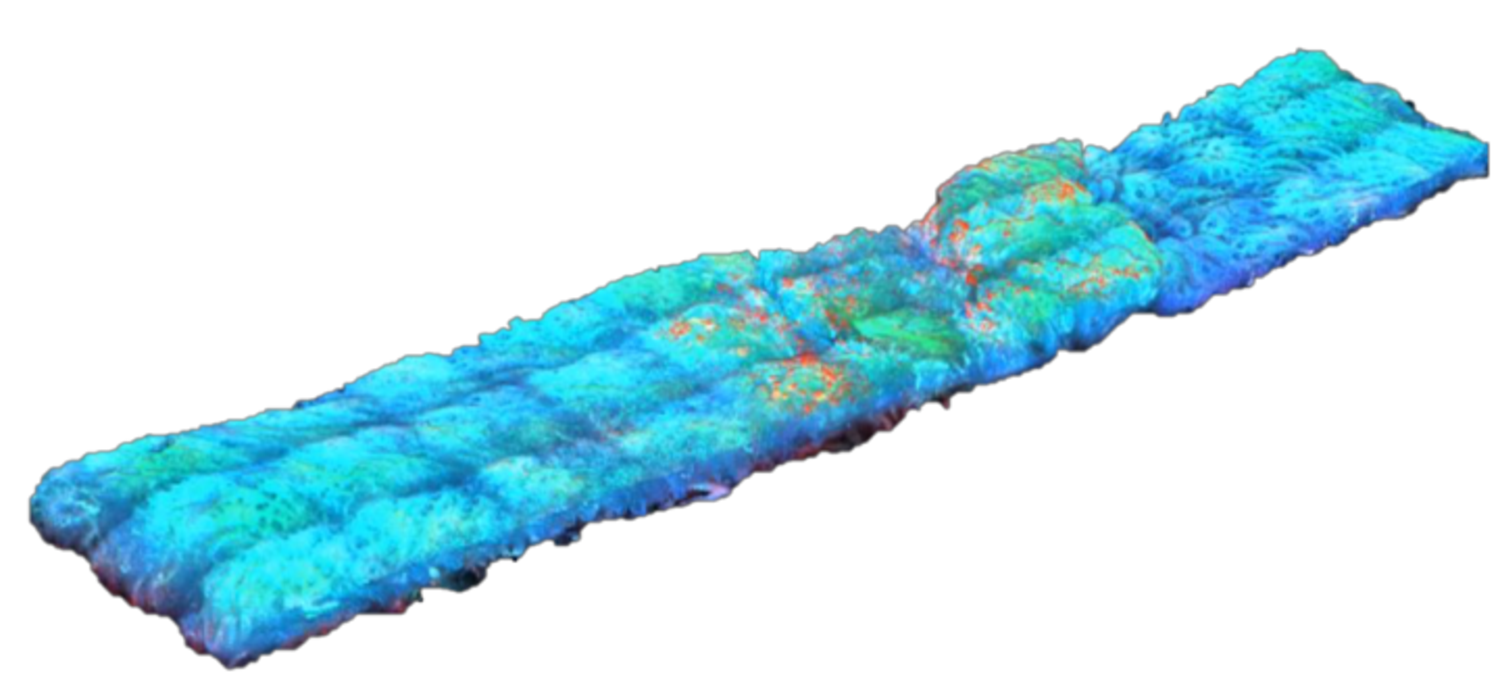
\includegraphics[clip, width=\linewidth]{fig/chapter3/3d_samples/sample_A_clip}
		\subcaption{sample A}
	\end{minipage}
	\begin{minipage}{0.45\linewidth}
		\centering
		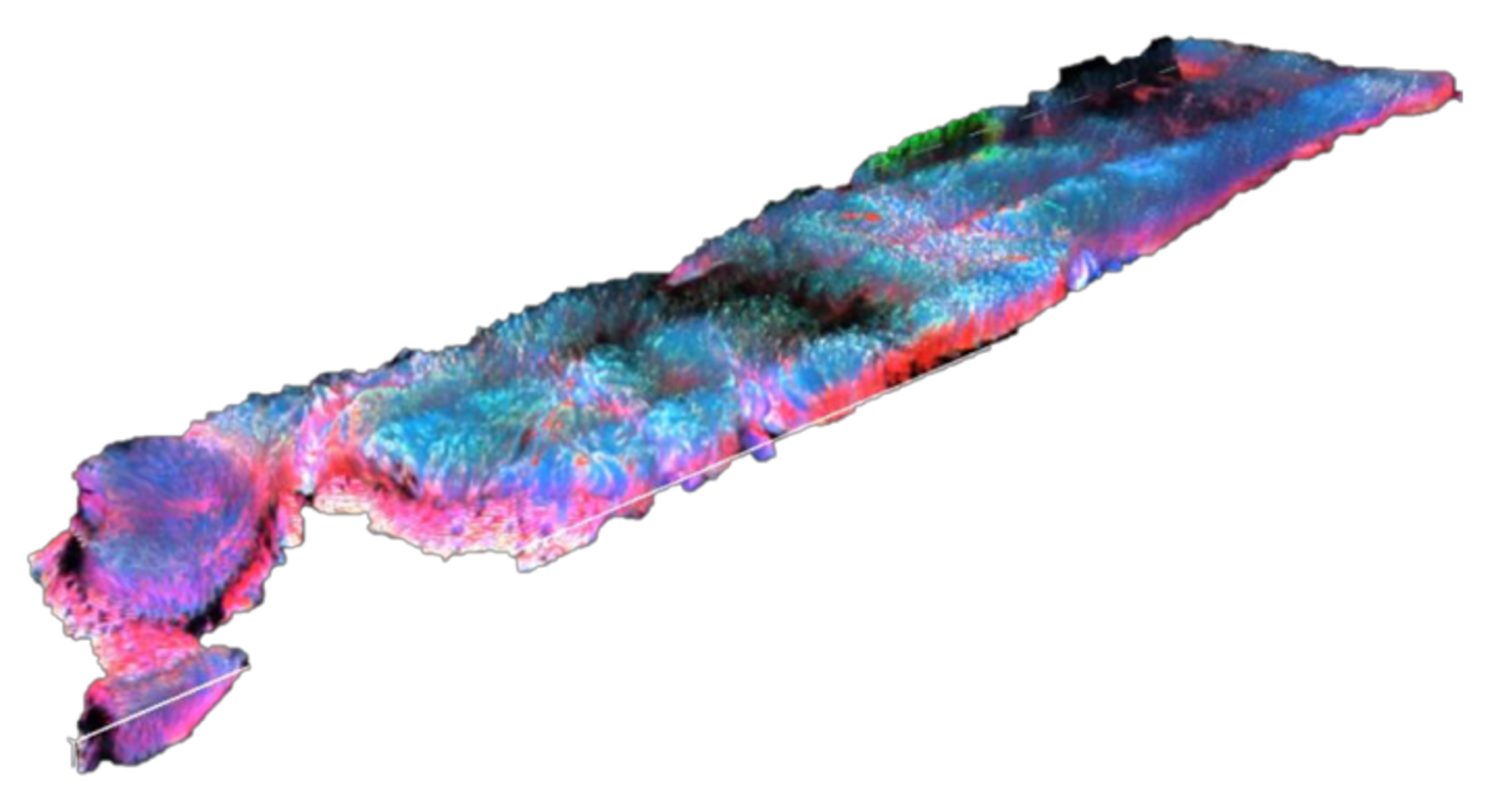
\includegraphics[clip, width=\linewidth]{fig/chapter3/3d_samples/sample_B_clip}
		\subcaption{sample B}
	\end{minipage}
	\begin{minipage}{0.45\columnwidth}
		\centering
		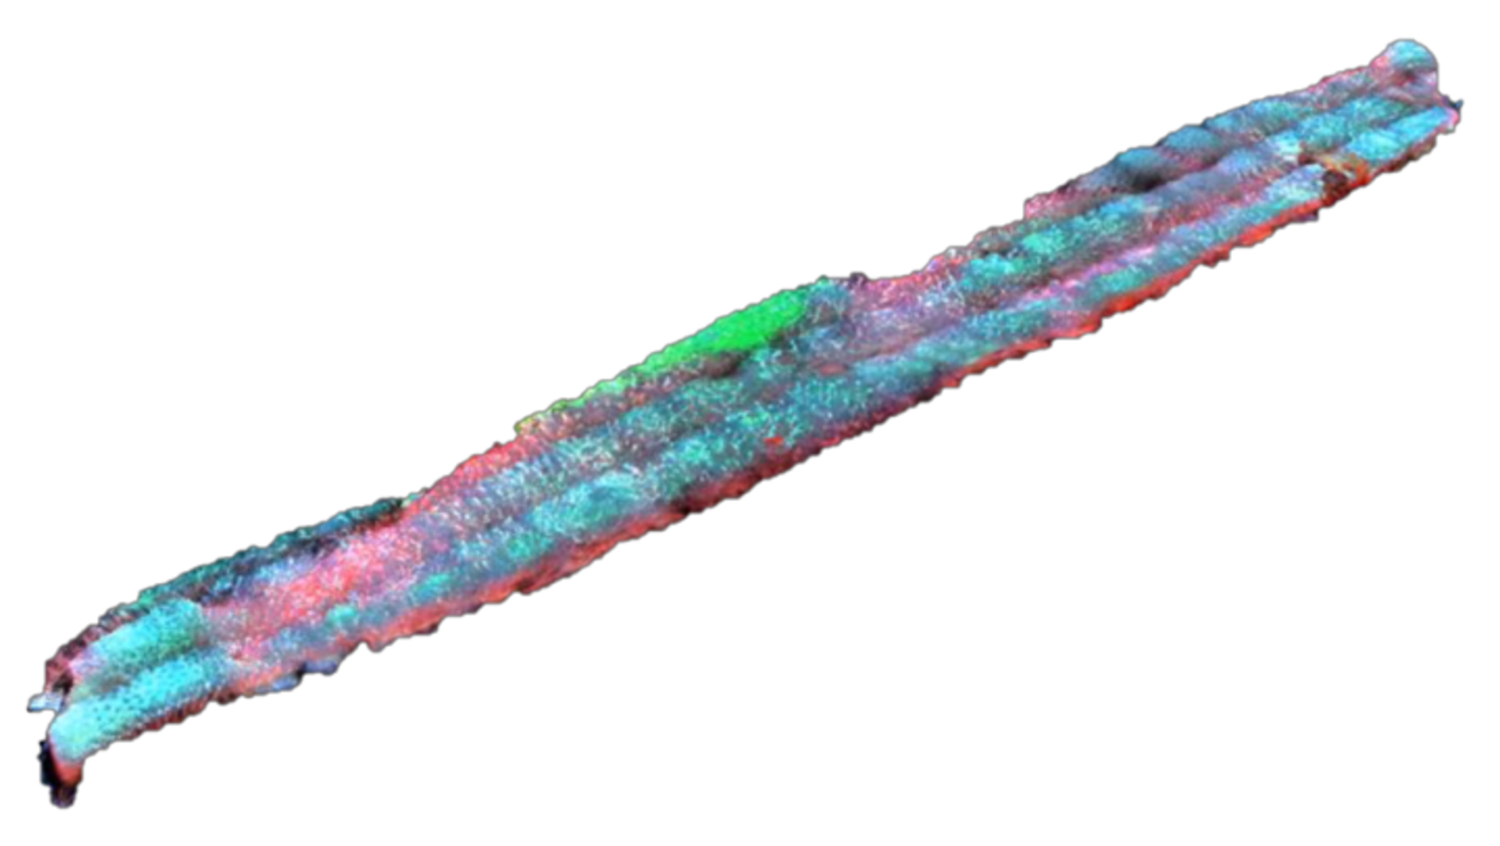
\includegraphics[clip, width=\linewidth]{fig/chapter3/3d_samples/sample_C_clip}
		\subcaption{sample C}
	\end{minipage}
	\begin{minipage}{0.45\linewidth}
		\centering
		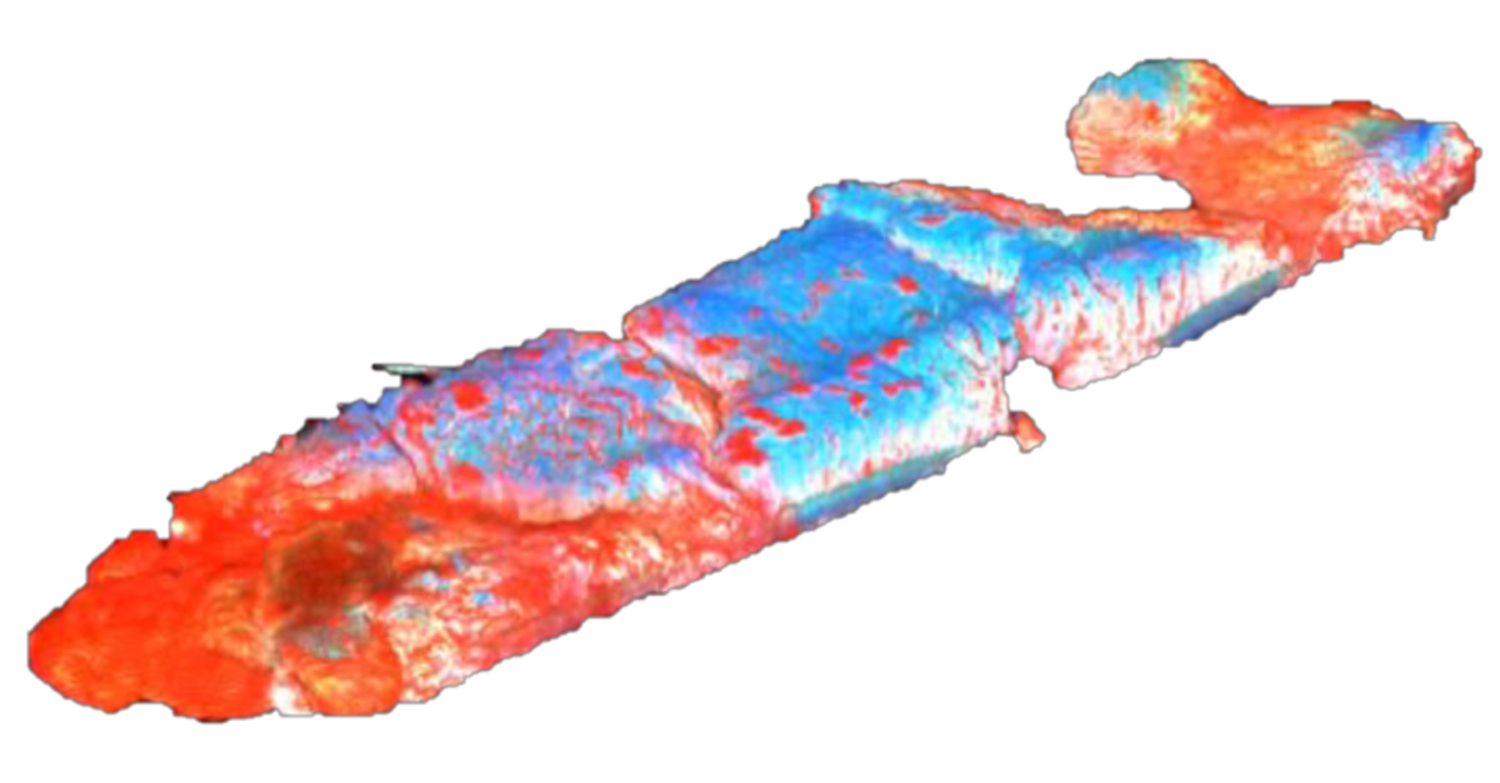
\includegraphics[clip, width=\linewidth]{fig/chapter3/3d_samples/sample_D_clip}
		\subcaption{sample D}
	\end{minipage}
	
	\caption{Overview samples}
	\label{fig:3D検体一覧}
	
\end{figure}


\fig {検体アノテーション}に専門医によって腫瘍をアノテーションした検体を示す.なお,検体Bのアノテーション画像はなかったため,共焦点レーザー顕微鏡の撮影像のみを載せた.

% アノテーション
\begin{figure}[H]
	\centering
	
	\begin{minipage}{0.45\columnwidth}
		\centering
		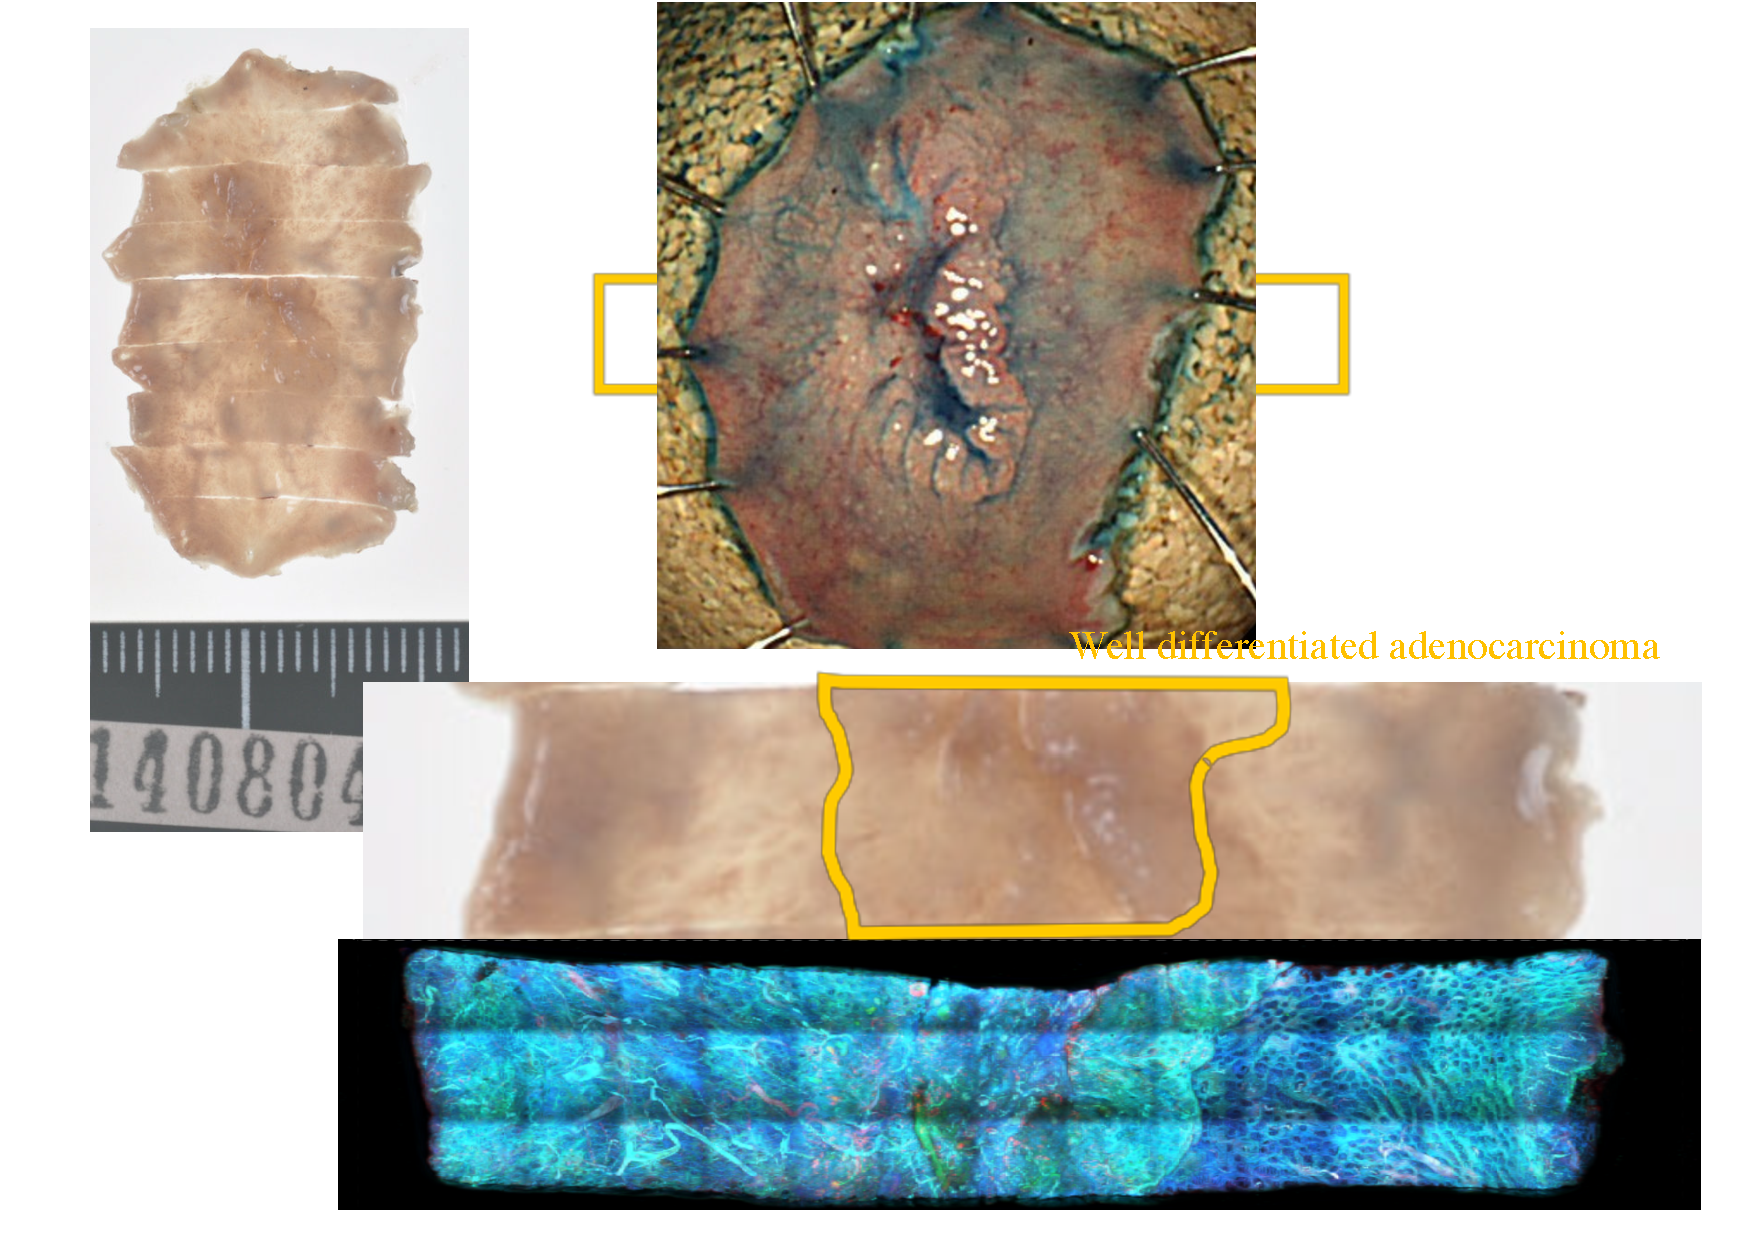
\includegraphics[clip, angle=270, width=\linewidth]{fig/raw_data/summary/C-013}
		\subcaption{sample A}
	\end{minipage}
	\begin{minipage}{0.45\linewidth}
		\centering
		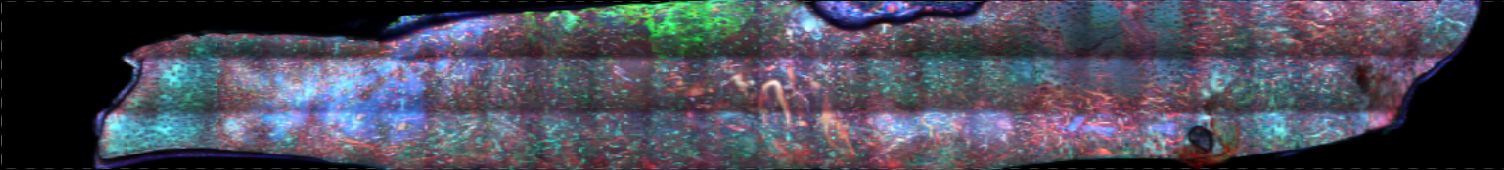
\includegraphics[clip, width=\linewidth]{fig/raw_data/summary/C-012}
		\subcaption{sample B}
	\end{minipage}
	\begin{minipage}{0.45\columnwidth}
		\centering
		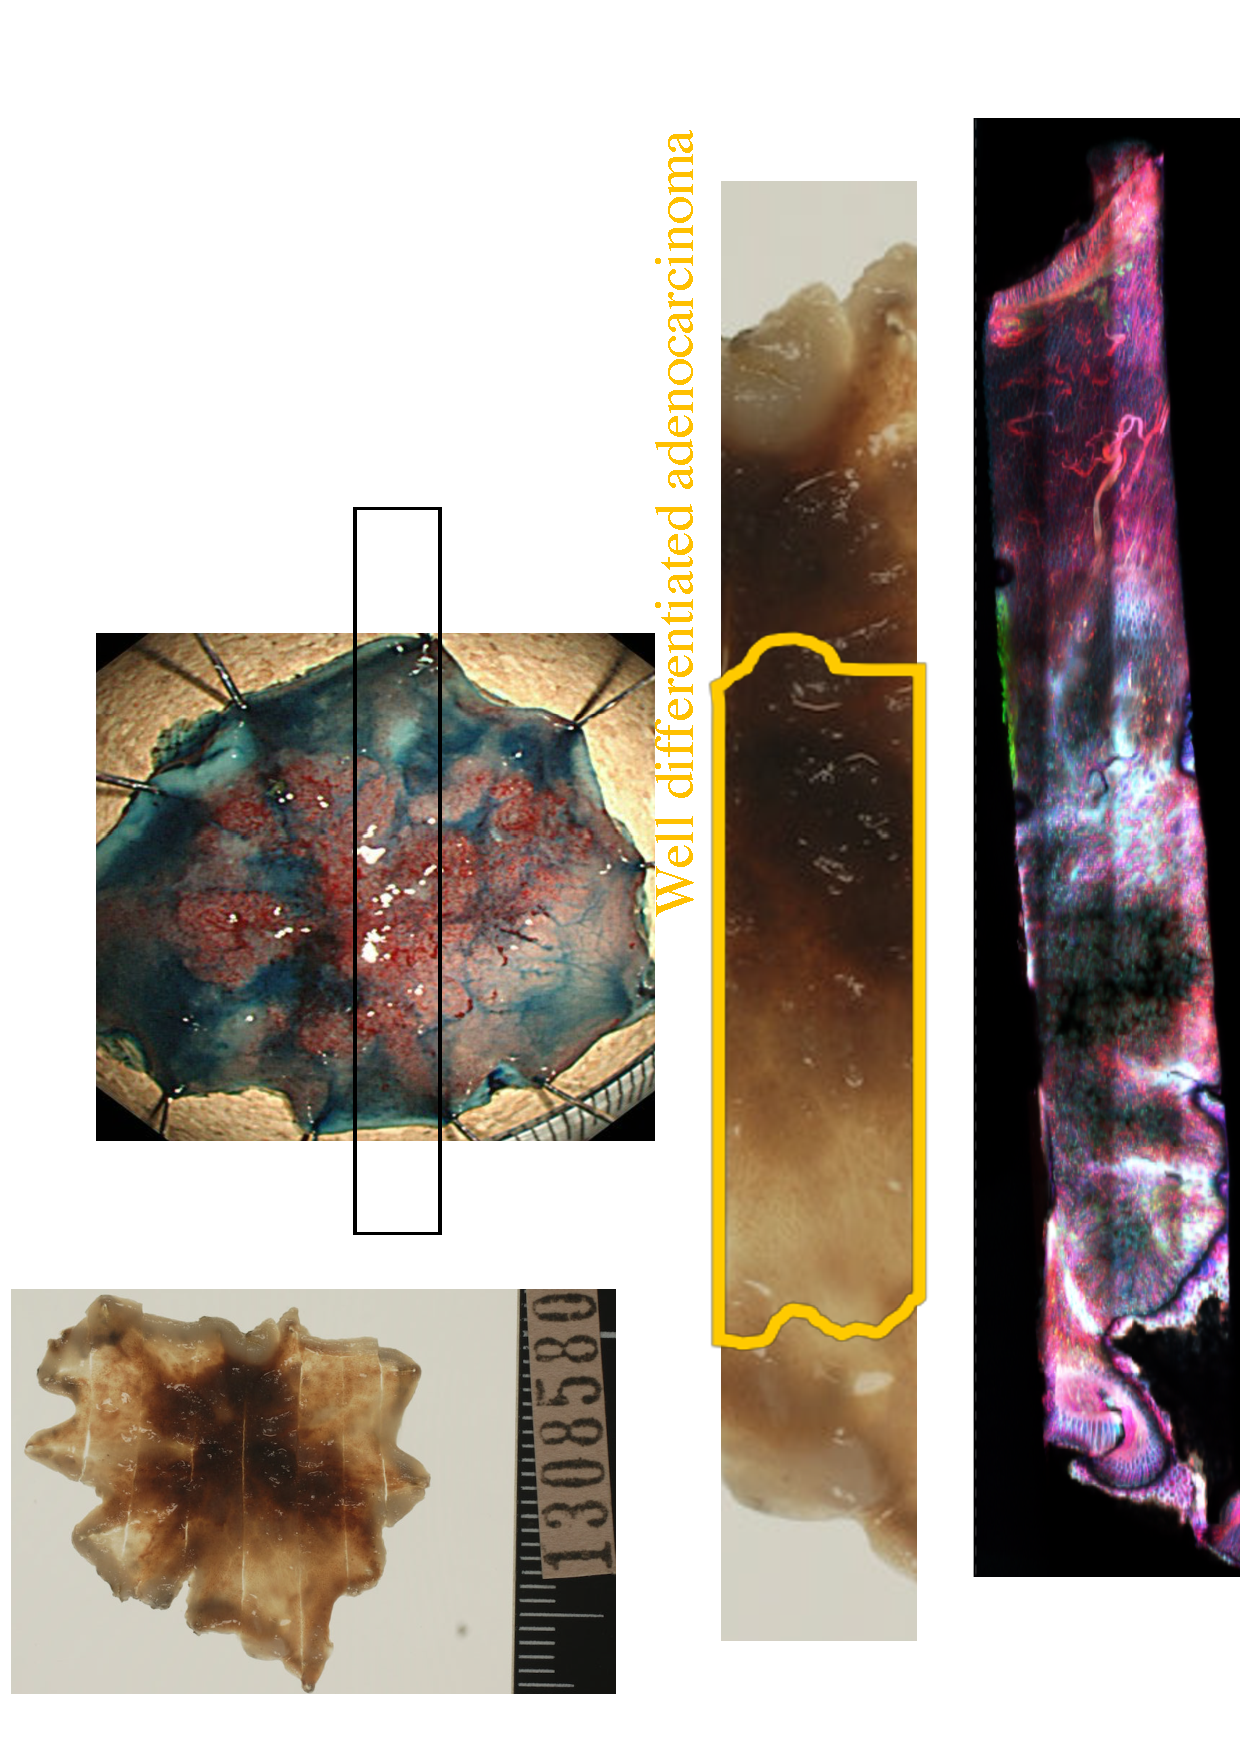
\includegraphics[clip, angle=270, width=\linewidth]{fig/raw_data/summary/C-009}
		\subcaption{sample C}
	\end{minipage}
	\begin{minipage}{0.45\linewidth}
		\centering
		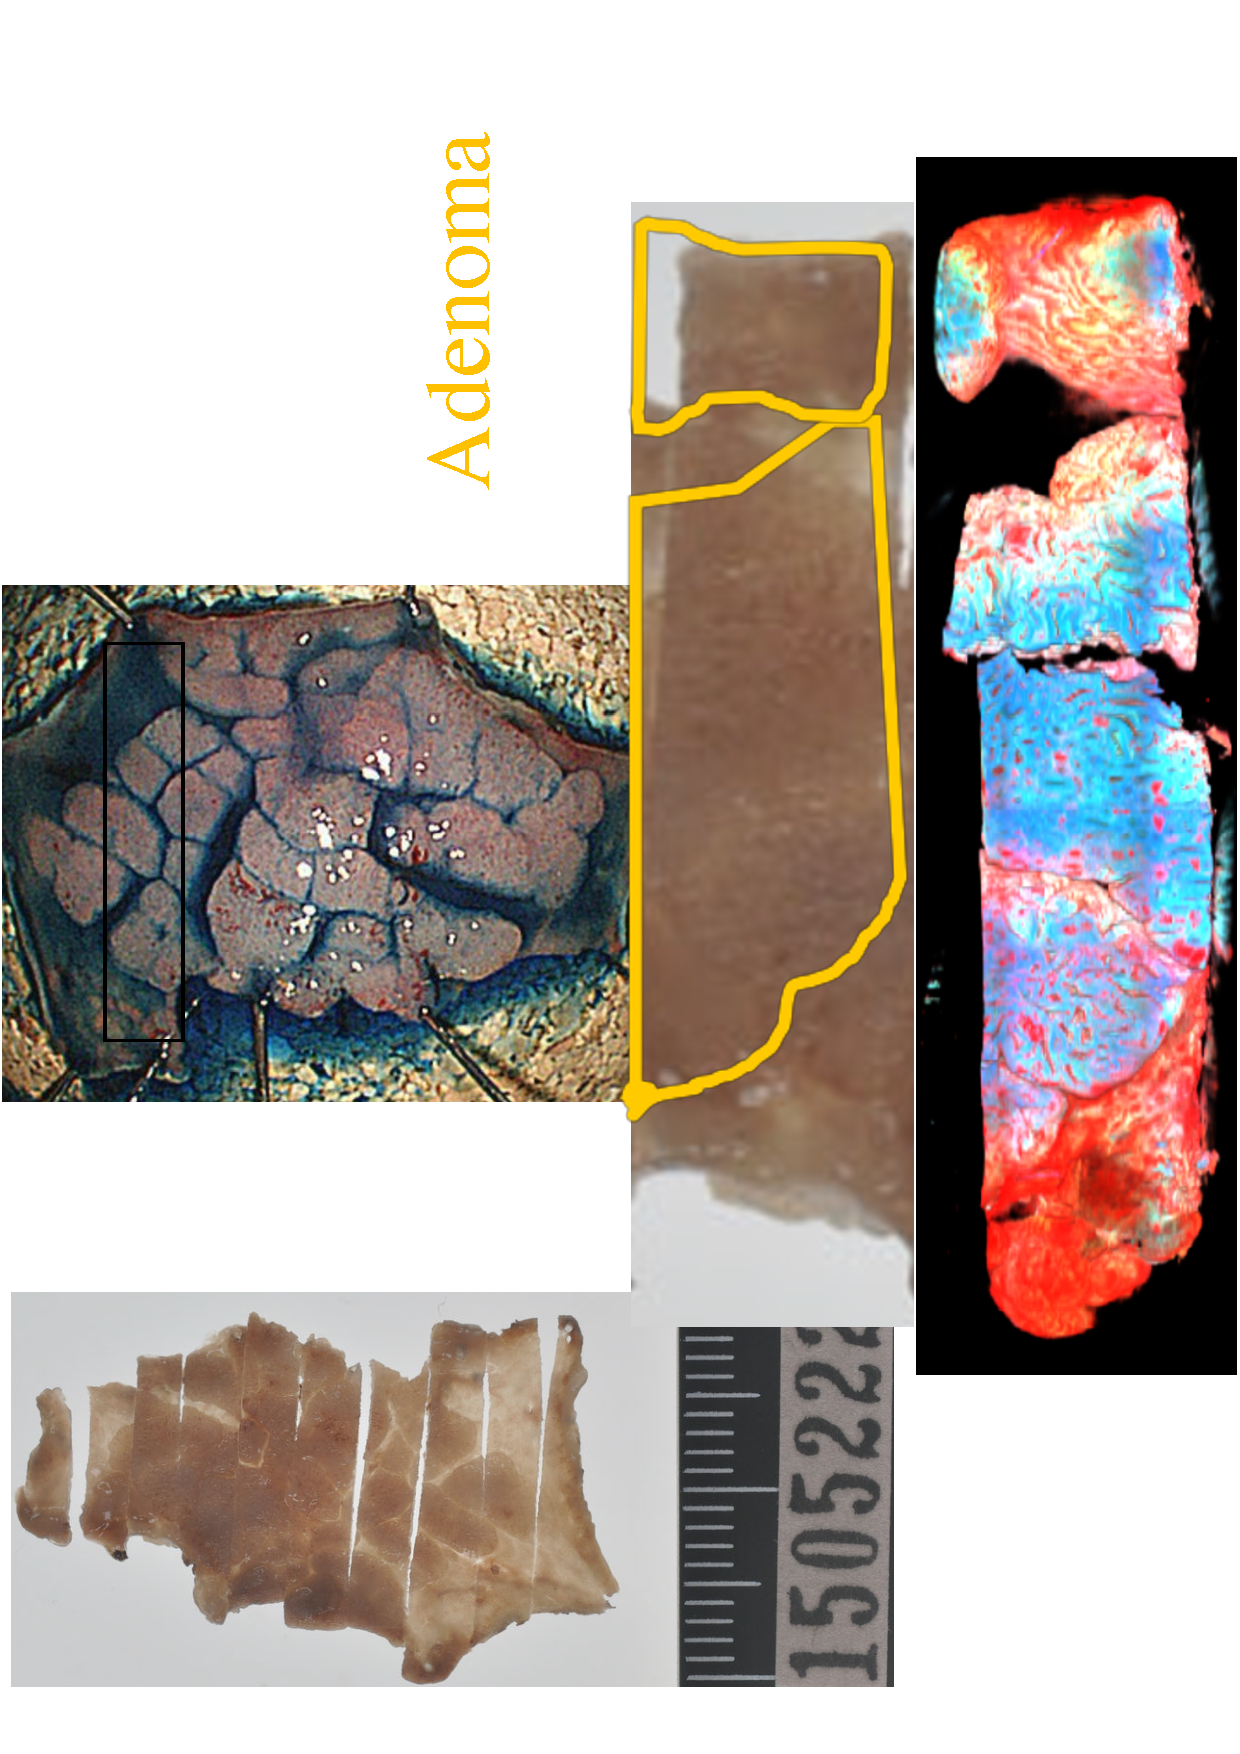
\includegraphics[clip, angle=270, width=\linewidth]{fig/raw_data/summary/C-011}
		\subcaption{sample D}
	\end{minipage}
	
	\caption{Annotation images of samples}
	\label{fig:検体アノテーション}
	
\end{figure}






\subsection{教師データの作成}
消化器内科の医師がつけた腫瘍部分を教師データとして利用した.\fig {切り取り画像}が腫瘍の位置をマスクした画像になっている.

\begin{figure}[H]
	\centering
	
	\begin{minipage}{0.8\columnwidth}
		\centering
		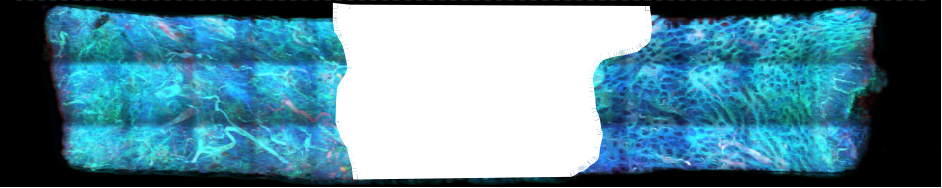
\includegraphics[clip, width=\linewidth]{fig/raw_data/label/C-013}
		\subcaption{sample A}
	\end{minipage}	
	
	\begin{minipage}{0.8\columnwidth}
		\centering
		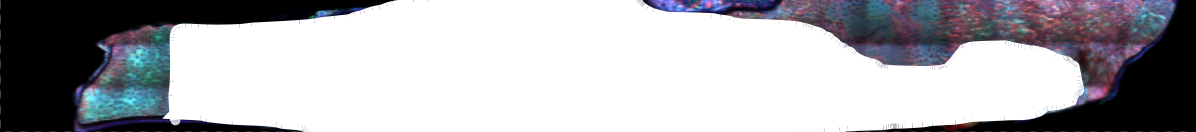
\includegraphics[clip, width=\linewidth]{fig/raw_data/label/C-012}
		\subcaption{sample B}
	\end{minipage}
	
	\begin{minipage}{0.8\columnwidth}
		\centering
		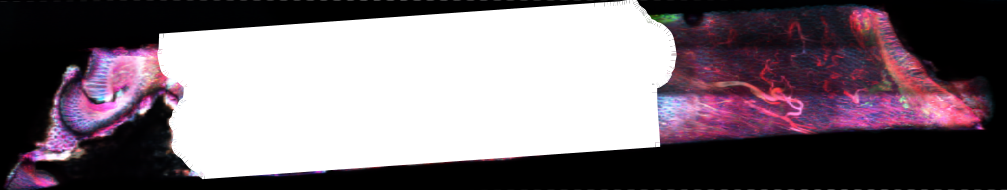
\includegraphics[clip, width=\linewidth]{fig/raw_data/label/C-009}
		\subcaption{sample C}
	\end{minipage}
	
	\begin{minipage}{0.8\columnwidth}
		\centering
		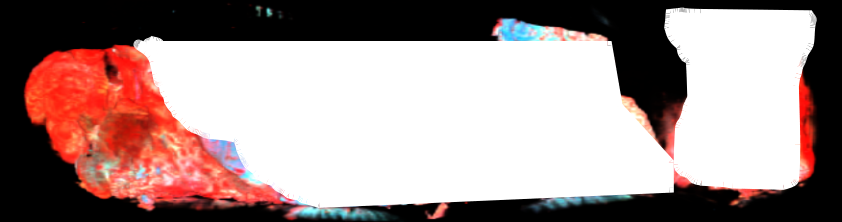
\includegraphics[clip, width=\linewidth]{fig/raw_data/label/C-011}
		\subcaption{sample D}
	\end{minipage}
	%\begin{minipage}{0.8\columnwidth}
	%	\centering
	%	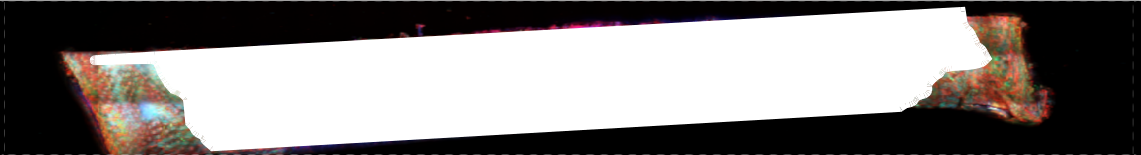
\includegraphics[clip, width=\linewidth]{fig/raw_data/label/C-010}
	%	\subcaption{sample E}
	%\end{minipage}
	
	\caption{Sample images masking cancer}
	\label{fig:切り取り画像}
	
\end{figure}


\section{前処理}
本研究では,学習器にかける前にいくつかの前処理を行った.本節ではこの前処理について述べる.

\subsection{擬似HE染色}
蛍光顕微鏡で撮影した画像は,病片発光色が検体ごとで異なるためそれらを一様に扱えない.そこで,病理でよく用いられるHE染色のカラーテイストへと変換した.
蛍光顕微鏡では,Texas Redで細胞核を染色し,DAPIで細胞質を青色に染色している.
従来の染色方法では,HE染色で,ヘマトキシリンが細胞核を染色して,エオジンで細胞質を染色している.したがって,蛍光顕微鏡をRGBに分割し,Rの画像をエオジンの紫色(121, 82, 147)に変換し,Bの色をヘマトキシリンのピンク色(245, 163, 237)に変換することで擬似HE染色の画像を作り出した.\fig {HElike}に示すように,全ての検体が同様な色調になっていることが分かる.

\begin{figure}[H]
	\centering
	
	\begin{minipage}{0.8\columnwidth}
		\centering
		\includegraphics[clip, angle=270, width=\linewidth]{fig/preprocessing/pseudo-HE/0130171}
		\subcaption{sample A}
	\end{minipage}
	\begin{minipage}{0.8\columnwidth}
		\centering
		\includegraphics[clip, angle=270, width=\linewidth]{fig/preprocessing/pseudo-HE/0120100}
		\subcaption{sample B}
	\end{minipage}
	\begin{minipage}{0.8\columnwidth}
		\centering
		\includegraphics[clip, angle=270, width=\linewidth]{fig/preprocessing/pseudo-HE/201901150050}
		\subcaption{sample C}
	\end{minipage}
	\begin{minipage}{0.8\columnwidth}
		\centering
		\includegraphics[clip, angle=270, width=\linewidth]{fig/preprocessing/pseudo-HE/0110240}
		\subcaption{sample D}
	\end{minipage}
	%\begin{minipage}{0.8\columnwidth}
	%	\centering
	%	\includegraphics[clip, angle=270, width=\linewidth]{fig/preprocessing/pseudo-HE/0100}
	%	\subcaption{sample E}
	%\end{minipage}
	
	\caption{Sample images preprocessing like HE}
	\label{fig:HElike}
	
\end{figure}


また\fig {切り取り画像}に示した教師ラベルから,画像データを正常と腫瘍に分割した.その一例を\fig {検体A教師ラベル}に示す.

\begin{figure}[H]
	\centering
	
	\begin{minipage}{0.4\columnwidth}
		\centering
		\includegraphics[clip, width=\linewidth]{fig/preprocessing/separated_label/normal/normal_C-013}
		\subcaption{Normal of sample A}
	\end{minipage}
	\begin{minipage}{0.4\columnwidth}
		\centering
		\includegraphics[clip, width=\linewidth]{fig/preprocessing/separated_label/cancer/cancer_C-013}
		\subcaption{Cancer of sample A}
	\end{minipage}
	
	\caption{Example of teacher labels of normal and cancer}
	\label{fig:検体A教師ラベル}
	
\end{figure}


\subsection{Data Augmentation}
本研究ではデータセットが少量である.そこで少しの画像からより多くの特徴を抽出するために,擬似的なデータの水増し(Data Augmentation)を行った.本研究で注意した点は,入力画像としてあり得る範囲のバリエーションに絞った点である.

Data Augmentationは1エポックごとに行われるので,訓練データは50エポック学習したら1つのData Augmentationに対して50倍にも増やすことができる.

\subsection*{回転}
入力画像を90\deg 刻みで最大270\deg 回転させた.その一例を\fig {回転}に示す.

\begin{figure}[H]
	\centering
	
	\begin{minipage}{0.24\columnwidth}
		\centering
		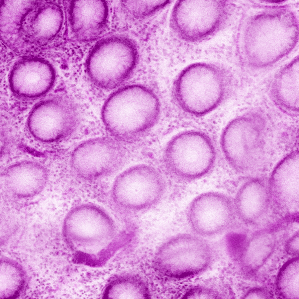
\includegraphics[clip, width=\linewidth]{fig/preprocessing/data_aug/rotate/ROTATION_0}
		\subcaption{0\deg}
	\end{minipage}
	\begin{minipage}{0.24\columnwidth}
		\centering
		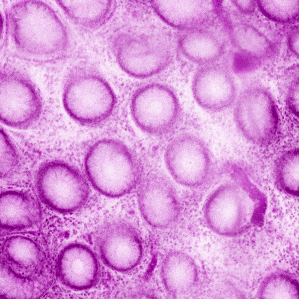
\includegraphics[clip, width=\linewidth]{fig/preprocessing/data_aug/rotate/ROTATION_90}
		\subcaption{90\deg}
	\end{minipage}
	\begin{minipage}{0.24\columnwidth}
		\centering
		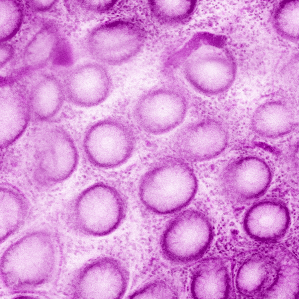
\includegraphics[clip, width=\linewidth]{fig/preprocessing/data_aug/rotate/ROTATION_180}
		\subcaption{180\deg}
	\end{minipage}
	\begin{minipage}{0.24\columnwidth}
		\centering
		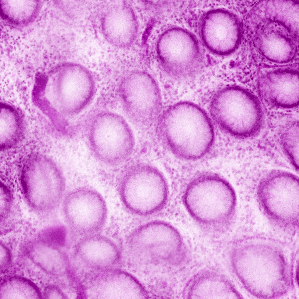
\includegraphics[clip, width=\linewidth]{fig/preprocessing/data_aug/rotate/ROTATION_270}
		\subcaption{270\deg}
	\end{minipage}
	
	\caption{Rotation}
	\label{fig:回転}
	
\end{figure}

\subsection*{反転}
入力画像を垂直方向および水平方向に反転させた.その一例を\fig {反転}に示す.

\begin{figure}[H]
	\centering
	
	\begin{minipage}{0.25\columnwidth}
		\centering
		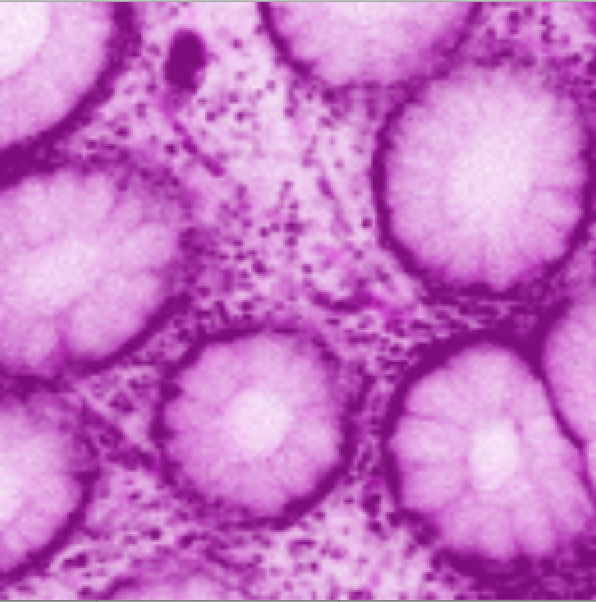
\includegraphics[clip, width=\linewidth]{fig/preprocessing/data_aug/horizontal_flip/horizontal_flip}
		\subcaption{horizontal flipping}
	\end{minipage}
	\begin{minipage}{0.1\columnwidth}
		\hspace{2truemm}
	\end{minipage}
	\begin{minipage}{0.25\columnwidth}
		\centering
		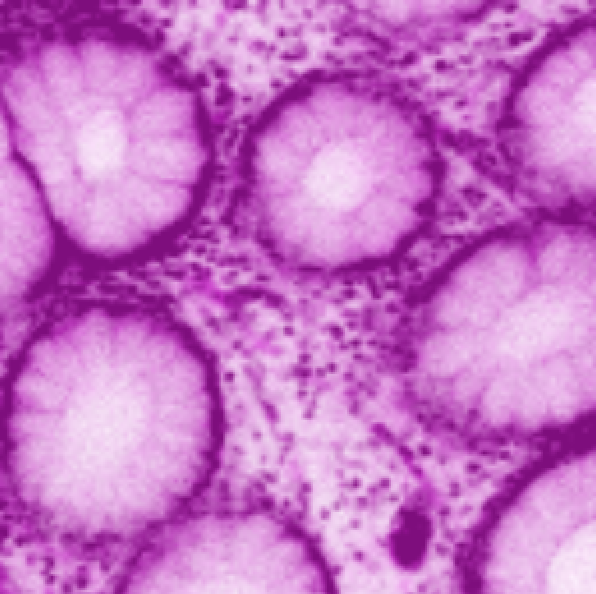
\includegraphics[clip, width=\linewidth]{fig/preprocessing/data_aug/vertical_flip/vertical_flip}
		\subcaption{vertical flipping}
	\end{minipage}
	
	\caption{Flipping}
	\label{fig:反転}
	
\end{figure}

\subsection*{ガウシアンブラー}
入力画像にぼかしを加えた.ぼかしにはガウシアンブラーを適用し,ぼかし半径は0.5刻みで最大2まで行った.その一例を\fig {ガウシアンブラー}に示す.

\begin{figure}[H]
	\centering
	
	\begin{minipage}{0.24\columnwidth}
		\centering
		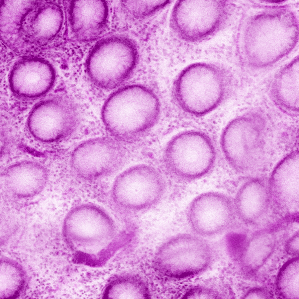
\includegraphics[clip, width=\linewidth]{fig/preprocessing/data_aug/color/blur/blur_0_00}
		\subcaption{$r=0$}
	\end{minipage}
	\begin{minipage}{0.24\columnwidth}
		\centering
		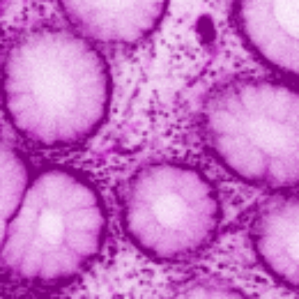
\includegraphics[clip, width=\linewidth]{fig/preprocessing/data_aug/color/blur/blur_0_50}
		\subcaption{$r=0.50$}
	\end{minipage}
	\begin{minipage}{0.24\columnwidth}
		\centering
		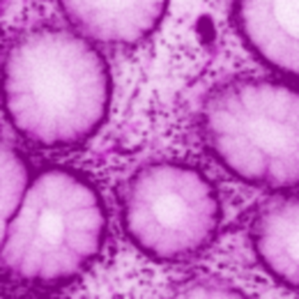
\includegraphics[clip, width=\linewidth]{fig/preprocessing/data_aug/color/blur/blur_1_00}
		\subcaption{$r=1.00$}
	\end{minipage}
	\begin{minipage}{0.24\columnwidth}
		\centering
		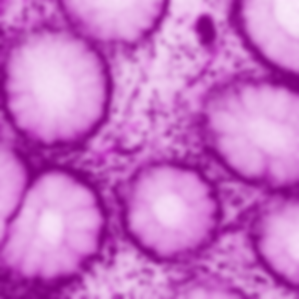
\includegraphics[clip, width=\linewidth]{fig/preprocessing/data_aug/color/blur/blur_2_00}
		\subcaption{$r=2.00$}
	\end{minipage}
	
	\caption{Gaussian blur. $r$ is blur radius.}
	\label{fig:ガウシアンブラー}
	
\end{figure}

\subsection*{鮮鋭度}
入力画像の鮮鋭度(シャープネス)を変えた.ここで$f$は使用したライブラリPillowのfactorで,最大$f=2.00$まで適用した.その一例を\fig {シャープネス}に示す.

\begin{figure}[H]
	\centering
	
	\begin{minipage}{0.24\columnwidth}
		\centering
		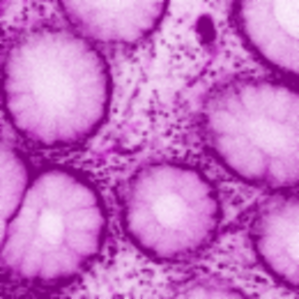
\includegraphics[clip, width=\linewidth]{fig/preprocessing/data_aug/color/SHARPNESS/SHARPNESS_0_00}
		\subcaption{$f=0$}
	\end{minipage}
	\begin{minipage}{0.24\columnwidth}
		\centering
		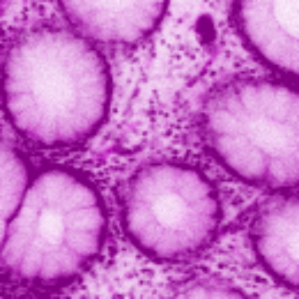
\includegraphics[clip, width=\linewidth]{fig/preprocessing/data_aug/color/SHARPNESS/SHARPNESS_0_50}
		\subcaption{$f=0.50$}
	\end{minipage}
	\begin{minipage}{0.24\columnwidth}
		\centering
		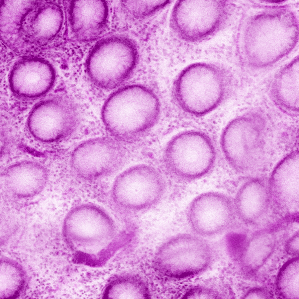
\includegraphics[clip, width=\linewidth]{fig/preprocessing/data_aug/color/SHARPNESS/SHARPNESS_1_00}
		\subcaption{$f=1.00$}
	\end{minipage}
	\begin{minipage}{0.24\columnwidth}
		\centering
		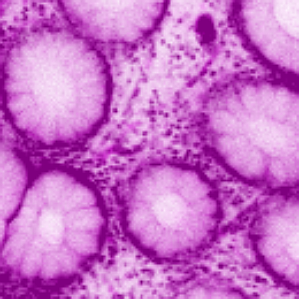
\includegraphics[clip, width=\linewidth]{fig/preprocessing/data_aug/color/SHARPNESS/SHARPNESS_2_00}
		\subcaption{$f=2.00$}
	\end{minipage}
	
	\caption{Sharpness. $f$ is enhancement factor. An enhancement factor of 0.0 gives a blurred image, a factor of 1.0 gives the original image, and a factor of 2.0 gives a sharpened image.}
	\label{fig:シャープネス}
	
\end{figure}

\subsection*{輝度}
入力画像の輝度(明るさ)を変えた.ここで$I$は輝度値であり,$I=1.00$が元の明るさで,$I=1.20$は1.2倍の明るく,$I=0.80$は0.8倍暗くなっている.その一例を\fig {輝度}に示す.

\begin{figure}[H]
	\centering
	
	\begin{minipage}{0.25\columnwidth}
		\centering
		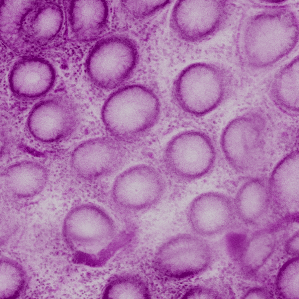
\includegraphics[clip, width=\linewidth]{fig/preprocessing/data_aug/color/BRIGHTNESS/BRIGHTNESS_0_80}
		\subcaption{$I=0.80$}
	\end{minipage}
	\begin{minipage}{0.25\columnwidth}
		\centering
		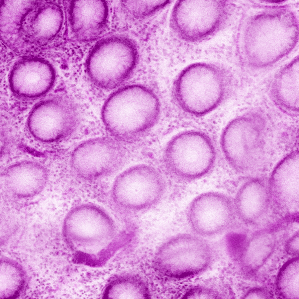
\includegraphics[clip, width=\linewidth]{fig/preprocessing/data_aug/color/BRIGHTNESS/BRIGHTNESS_1_00}
		\subcaption{$I=1.00$}
	\end{minipage}
	\begin{minipage}{0.25\columnwidth}
		\centering
		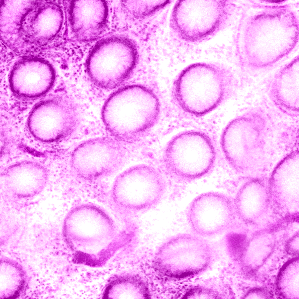
\includegraphics[clip, width=\linewidth]{fig/preprocessing/data_aug/color/BRIGHTNESS/BRIGHTNESS_1_20}
		\subcaption{$I=1.20$}
	\end{minipage}
	
	\caption{Intensity. $I$ is intensity of RGB color. An intensity of 0.0 gives a black image. An intensity of 1.0 gives the original image.}
	\label{fig:輝度}
	
\end{figure}

\subsection*{コントラスト}
入力画像のコントラストを変えた.ここで$f$は使用したライブラリPillowのfactorで,最大$f=1.50$まで適用した.その一例を\fig {コントラスト}に示す.

\begin{figure}[H]
	\centering
	
	\begin{minipage}{0.25\columnwidth}
		\centering
		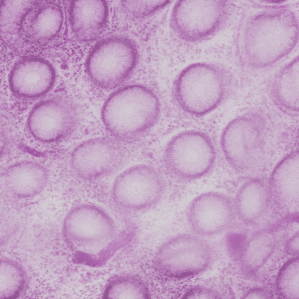
\includegraphics[clip, width=\linewidth]{fig/preprocessing/data_aug/color/CONTRAST/CONTRAST_0_50}
		\subcaption{$f = 0.50$}
	\end{minipage}
	\begin{minipage}{0.25\columnwidth}
		\centering
		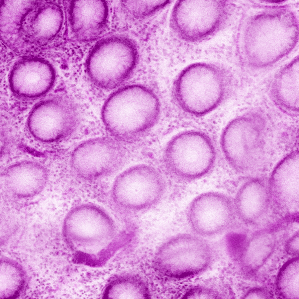
\includegraphics[clip, width=\linewidth]{fig/preprocessing/data_aug/color/CONTRAST/CONTRAST_1_00}
		\subcaption{$f = 1.00$}
	\end{minipage}
	\begin{minipage}{0.25\columnwidth}
		\centering
		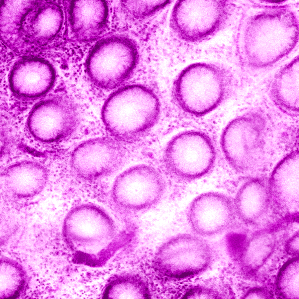
\includegraphics[clip, width=\linewidth]{fig/preprocessing/data_aug/color/CONTRAST/CONTRAST_1_50}
		\subcaption{$f = 1.50$}
	\end{minipage}	
	
	\caption{Contrast. $f$ is enhancement factor. An enhancement factor of 0.0 gives a solid grey image. A factor of 1.0 gives the original image.}
	\label{fig:コントラスト}
	
\end{figure}

\subsection*{彩度}
入力画像の彩度を変えた.ここで$f$は使用したライブラリPillowのfactorで,最大$f=1.50$まで適用した.その一例を\fig {彩度}に示す.

\begin{figure}[H]
	\centering
	
	\begin{minipage}{0.25\columnwidth}
		\centering
		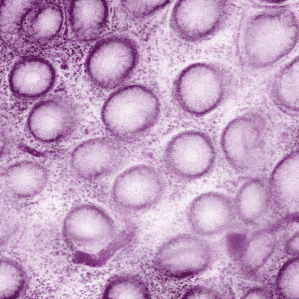
\includegraphics[clip, width=\linewidth]{fig/preprocessing/data_aug/color/SATURATION/SATURATION_0_50}
		\subcaption{$f = 0.50$}
	\end{minipage}
	\begin{minipage}{0.25\columnwidth}
		\centering
		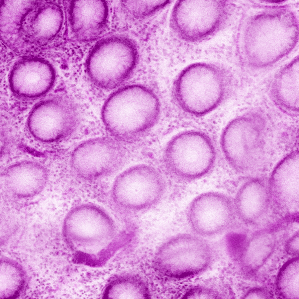
\includegraphics[clip, width=\linewidth]{fig/preprocessing/data_aug/color/SATURATION/SATURATION_1_00}
		\subcaption{$f = 1.00$}
	\end{minipage}
	\begin{minipage}{0.25\columnwidth}
		\centering
		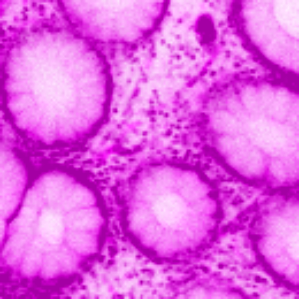
\includegraphics[clip, width=\linewidth]{fig/preprocessing/data_aug/color/SATURATION/SATURATION_1_50}
		\subcaption{$f = 1.50$}
	\end{minipage}	
	
	\caption{Saturation. $f$ is enhancement factor. An enhancement factor of 0.0 gives a black and white image. A factor of 1.0 gives the original image.}
	\label{fig:彩度}
	
\end{figure}

\subsection*{ランダムクロッピング}
これまでの画像のサイズは,$299 \times 299$であったが,この画像からランダムな場所で$256 \times 256$に切り抜き(クロッピング)を行う.訓練画像はランダムで切り抜くが,テスト画像では,中心を$256 \times 256$に切り抜く.

\begin{figure}[H]
	\centering
	
	\begin{minipage}{0.25\columnwidth}
		\centering
		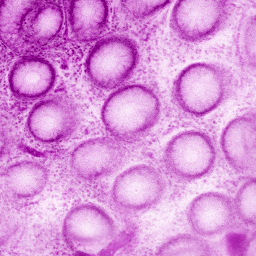
\includegraphics[clip, width=\linewidth]{fig/preprocessing/data_aug/random_crop/x0_y0}
		\subcaption{crop left}
	\end{minipage}
	\begin{minipage}{0.25\columnwidth}
		\centering
		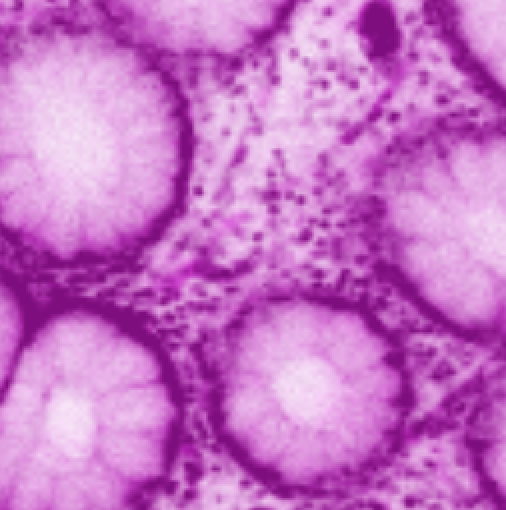
\includegraphics[clip, width=\linewidth]{fig/preprocessing/data_aug/random_crop/x15_y15}
		\subcaption{crop center}
	\end{minipage}
	\begin{minipage}{0.25\columnwidth}
		\centering
		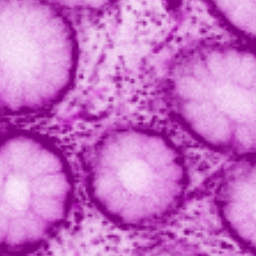
\includegraphics[clip, width=\linewidth]{fig/preprocessing/data_aug/random_crop/x34_y34}
		\subcaption{crop right}
	\end{minipage}	
	
	\caption{Random Cropping}
	\label{fig:ランダムクロッピング}
	
\end{figure}

\subsection{テスト画像}
入力画像の中心を$130\times 130$ pixでクロッピングし,これをテストデータとした.\fig {クロップ}に各検体のクロッピング画像を示す.

\begin{figure}[H]
	\centering
	
	\begin{minipage}{0.45\columnwidth}
		\centering
		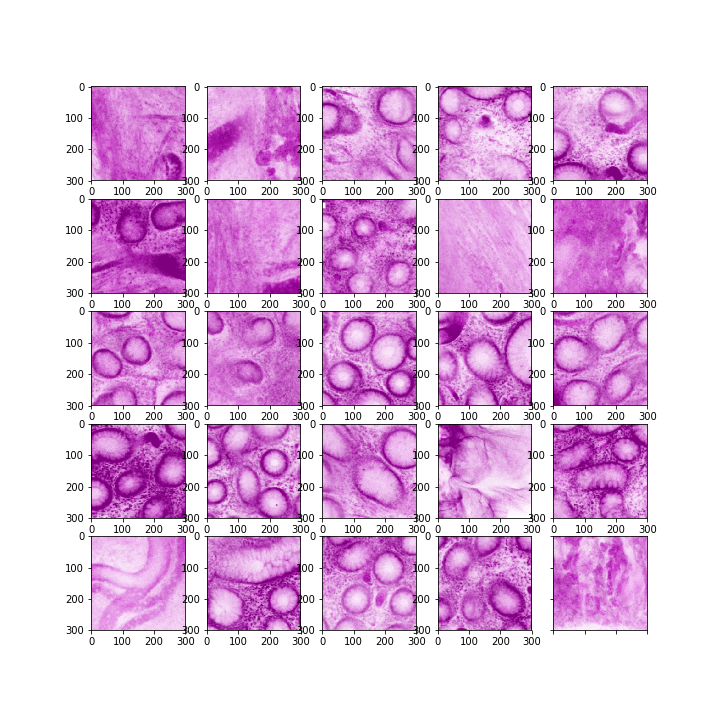
\includegraphics[clip, width=\linewidth]{fig/preprocessing/cropping/HE/normal/C-013}
		\subcaption{Normal images of sample A}
	\end{minipage}
	\begin{minipage}{0.45\columnwidth}
		\centering
		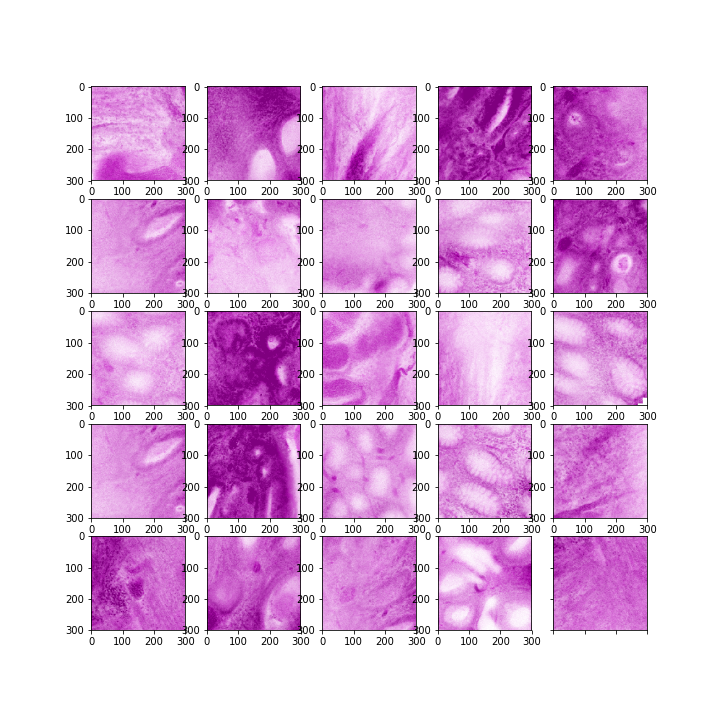
\includegraphics[clip, width=\linewidth]{fig/preprocessing/cropping/HE/cancer/C-013}
		\subcaption{Cancer images of sample A}
	\end{minipage}
	
	\begin{minipage}{0.45\columnwidth}
		\centering
		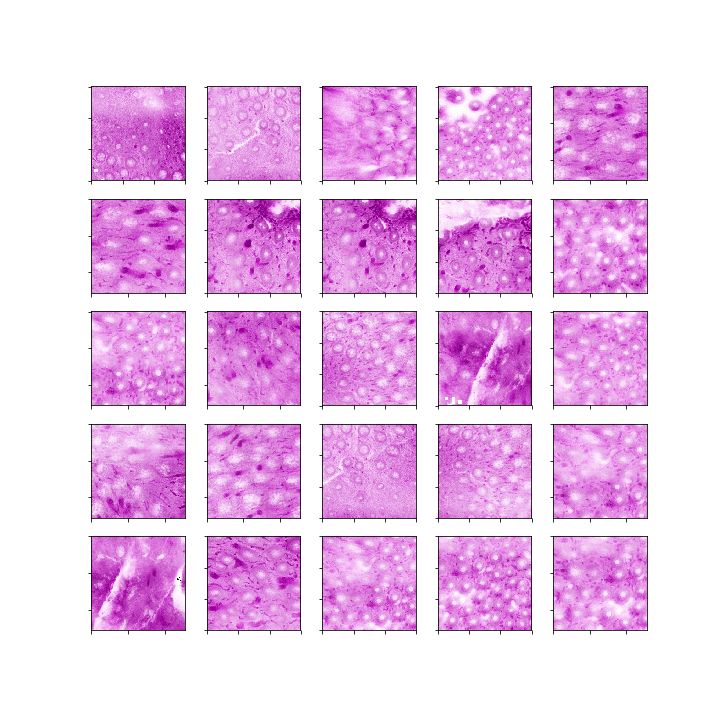
\includegraphics[clip, width=\linewidth]{fig/preprocessing/cropping/HE/normal/C-012}
		\subcaption{Normal images of sample B}
	\end{minipage}
	\begin{minipage}{0.45\columnwidth}
		\centering
		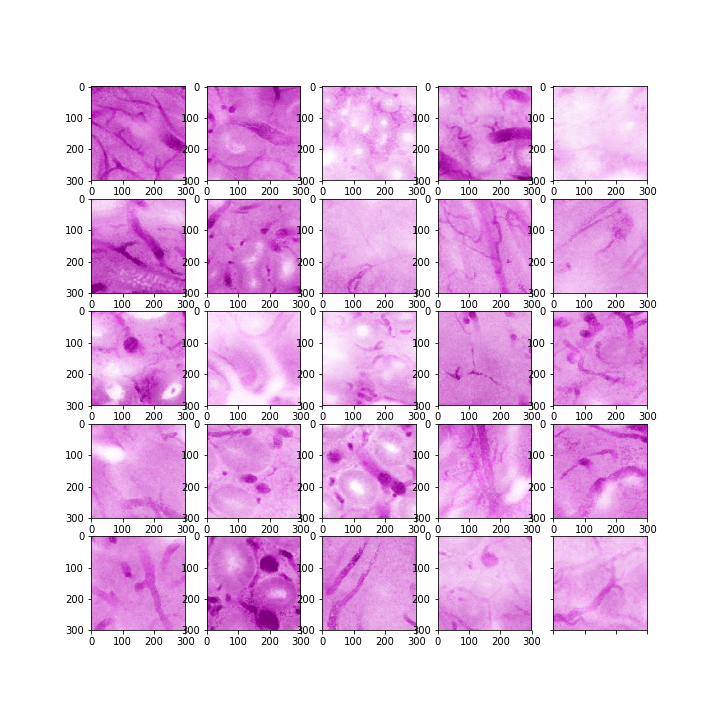
\includegraphics[clip, width=\linewidth]{fig/preprocessing/cropping/HE/cancer/C-012}
		\subcaption{Cancer images of sample B}
	\end{minipage}
	
	\caption{Cropped images for validation}
	\label{fig:クロップ}
	
\end{figure}

\section{古典的な画像処理手法による識別精度評価}
正常と腫瘍を両方含む画像に対して,Hough変換による円検出で正常の腺管構造を検出した.円検出では検出できない腺管構造をより多く検出するために,楕円でも検出ができるように変更した.複数のパラメータを調整することで,アノテーションの正常領域が検出できるような円検出の数を増やしながらも,ノイズが多くならないような値を決定した.また,これを複数の検体で試してみた時の最適なパラメータを見積もった.

\section{事前学習}
本研究では,新しい画像の撮影方法でデータを多く集めることができない.そこで,類似データを事前に学習しておく事前学習が有効であると考えた.今回,大腸の管構造の特徴を捉えるために,外部のデータセットであるGland Challengeデータセットを使って事前学習を行った.Gland Chellengeの詳細を\tab {GlandChallenge}に示す.

\begin{table}[H]
	\centering
	\caption{Data description}
	\label{tab:GlandChallenge}
	\begin{tabular}{cc}\toprule
		Cancer Type & Colorectal Cancer \\ 
		Resolution & $20\times (0.62005 \upmu \mathrm{m / pixel})$ \\ 
		Number of Images & 165 \\ 
		Format & bmp \\ \bottomrule
	\end{tabular} 
\end{table}


\begin{figure}[H]
	\centering
	
	\begin{minipage}[b]{0.4\columnwidth}
		\centering
		\includegraphics[clip, width=\linewidth]{fig/chapter2/pretrain_image/testA_5.bmp}
		\subcaption{Normal}
	\end{minipage}
	\hspace{5truemm}	
	\begin{minipage}[b]{0.4\columnwidth}
		\centering
		\includegraphics[clip, width=\linewidth]{fig/chapter2/pretrain_image/testA_12.bmp}
		\subcaption{Cancer}
	\end{minipage}
	
	\caption{Example of images for pre-training}
	\label{fig:事前学習画像}
	
\end{figure}

事前学習で用意する画像と本研究で使用する検体が類似ように,両方のデータセットに対して前処理を行った.

まず,両データの解像度を揃え,サンプル間で画像を正規化をした.事前学習の画像が,本検体の画像よりも解像度が4倍あった.事前学習のデータセットは画像サイズが異なるデータも多少あったため,画像サイズが$755 \times 522$ pixである画像151枚を利用し,その画像を$432 \times 299$ pixにリサイズした.また,本研究の検体をウィンドウサイズが130 pixとなるようにスライドウィンドウで画像を取得した.その際,背景の割合が0.1\%以上あるものは取り除いた.130 pixで切り抜いた画像を299 pixにリサイズして入力画像とした.
学習に用いる際には,事前学習の画像では$432 \times 299$ pixから$256 \times 256$ pixに切り抜き,本研究の検体では$299 \times 299$ pixをランダムに$256 \times 256$ pixに切り抜いて学習の教師データとした.


\section{教師あり学習による識別精度評価}
% モデルの概略図

\subsection{評価方法}
機械学習の評価方法には,ホールドアウト法と交差検証法の2通りある.ホールドアウト法は,あらかじめデータを訓練データとテストデータに分割して評価する方法である.交差検証法はデータを$K$分割して$K-1$のグループを訓練データに,残りの1つをテストデータにする.これを$K$パターン全て試行した精度の平均で評価する方法である.交差検証法の方が計算時間が長くなるが信頼性が高い.少量のデータの場合は訓練データとテストデータの分割の違いで結果に差が生じることがあるため,本研究の評価方法では交差検証法を用いた.

本研究では4検体を使っているため検体ごとに分割することで4分割の交差検証法を行った.

\subsection*{2次元画像}
用いたネットワーク構造は,InceptionV3,Xception,Inception-Resnetの4つである.
それぞれに対して,事前学習,擬似HE変換のあり・なしで精度がどのように改善されるかを実験した.

\subsection*{3次元画像}
深さ方向は10枚, 50枚,100枚の3パターンで3次元画像として解析した.用いたモデルは,擬似HE変換をした画像を事前学習で訓練した2DCNNのモデルをLSTM, GRU, Bidirectional-GRUの3つのモデルを検証した.


\section{教師なし学習による識別精度評価}
Autoencoder,GAN,VAE,を利用して教師なし学習を行った.Auto EncoderとGANは,生成画像が入力画像と類似するかを実験し,VAEでは,教師なし学習から得られる潜在変数の2次元平面への写像をした.また正常と腫瘍のそれぞれの画像が潜在変数の2次元空間で,構造的な違いからカテゴリーに分かれるかを確認した.


\section{半教師あり学習による識別精度評価}
VAEを利用して,\fig{半教師}のような半教師あり学習のネットワークを作成した.

\begin{figure}[H]
	\centering
	\begin{minipage}{\columnwidth}
		\centering
		\includegraphics[width=0.7\linewidth]{fig/chapter3/networks/patern_A}
		\subcaption{Not including teacher label}
		\label{fig:VAE-a}
	\end{minipage}
	
	\begin{minipage}{\columnwidth}
		\centering
		\includegraphics[width=0.7\linewidth]{fig/chapter3/networks/patern_B}
		\subcaption{Including teacher label}
		\label{fig:VAE-b}
	\end{minipage}
	
	\caption{Diagram of semi-supervised learning}
	\label{fig:半教師}
	
\end{figure}



\section{学習環境}
本研究の学習環境を\tab{環境}にまとめた.

\begin{table}[H]
	\centering
	\caption{Enviroment of implementation}
	\label{tab:環境}
	\begin{tabular}{ccc}\toprule
		OS & Ubuntu & ver. 14.04 \\ 
		Language & Python & ver. 3.6 \\ 
		\multirow{2}{*}{Framework} & Keras & ver. 2.2.4 \\ 
		& Tensorflow & ver. 1.11.0 \\ 
		GPU & GeForce GTX 1080Ti $\times$3 & RAM 11 GB \\  \bottomrule
	\end{tabular}
\end{table}

また,本研究で作成したプログラムはGithubに上げてある(下記URLを参照).\\
URL : 


\subsection*{バッチ学習}
本研究は3次元画像を解析するため,学習に利用する画像サイズやニューラルネットワークのパラメータ数が大きくなる.そのため本研究で使用したGPUではメモリに乗り切らないことがある.そこで画像をミニバッチに分けて,バッチごとに画像を読み込みGPUで計算を行った.
